\section{User Experience for mobiles}
<<<<<<< HEAD
<<<<<<< HEAD
\subsection{Introduction to user experience }
A study of user experience\footnote{hereafter referred to as UX} is a study of how a user feels when interacting with a system. The field encompasses a whole range of different and seemingly unrelated topics. The most known part of UX is probably the concept of usability which will be discussed later in the chapter, other things make up UX, such as: Design, Accessibility, System performance, Ergonomics, human factors and more concepts\todo{insert the source}. The term user experience  was originally coined by Dr. Donald Norman, who was the first to describe the importance of user-centered design. User-centered design is a design concept that lets the users dictate(to a certain degree) what the system should contain and what form it should take.
=======
=======
>>>>>>> parent of b7d1b95... Todays work on UX plus extra check description
The app that this project is aiming at developing will have a focus on the intuitive user experience. To have a focus on intuitiveness means that we must be able to understand what that implies. The dictionary defines intuitive as: 
\begin{itemize}
\item perceiving directly by intuition without rational thought, as a person or the mind.
\end{itemize}
they define the concept of intuitiveness as human perception by intuition, what then is intuition? again the dictionary will provide a relatively easy answer: 
\begin{itemize}
\item intuition\\
\begin{enumerate}
\item The act or faculty of perceiving, or apprehending by means of the senses or of the mind; cognition; understanding.
\item immediate or intuitive recognition or appreciation, as of moral, psychological, or aesthetic qualities; insight; intuition; discernment:
an artist of rare perception.
\item the result or product of perceiving, as distinguished from the act of perceiving; percept.
\item Psychology. a single unified awareness derived from sensory processes while a stimulus is present.
\end{enumerate}
\end{itemize} from this definition it is clear that the concept of intuitiveness is a human concept, more specifically a human psyche concept. In an article from 1994 Jef Raskin\cite{JRaskin} talks about how intuitiveness comes from familiarity, while the article is quite old the observations that he makes does support the idea that intuitiveness is directly linked with the targeted users. In the article Raskin talks about an experiment that he performed, where he gives asks a test participant to perform a certain task with a mouse, back in 1994 the mouse was still not a tool that was commonplace and as such the test subject had no familiarity with how to work with a mouse, and required help. Raskin showed the participant how to move the mouse in the correct manner, and instantly the participant knew how it worked and didnt require any more help, because as Raskin notes: \textit{"The directional mapping of the mouse was "intuitive" because in this regard it operated just like joysticks (to say nothing of pencils) with which she} [The test participant] \textit{was familiar"}\cite{JRaskin} this observation strongly supports the idea of "familiar equals intuitive"



 This section will first give brief overview of the topic of user experience. Next the section try and define what the intuitive user experience is, and lastly how does the gained knowledge translate to being used as guidelines for making an intuitive mobile device app.  

\subsection{Introduction to user experience }
A study of user experience\footnote{hereafter referred to as UX} is a study of how a user feels when interacting with a system. The field encompasses a whole range of different and seemingly unrelated topics. The most known part of UX is probably the concept of usability which will be discussed later in the chapter, other things make up UX, such as: Design, Accessibility, System performance, Ergonomics, human factors and more concepts\cite{UXIntro}. The term user experience  was originally coined by Dr. Donald Norman, who was the first to describe the importance of user-centered design. User-centered design is a design concept that lets the users dictate(to a certain degree) what the system should contain and what form it should take.
<<<<<<< HEAD
>>>>>>> parent of b7d1b95... Todays work on UX plus extra check description
=======
>>>>>>> parent of b7d1b95... Todays work on UX plus extra check description
Before user-centered design the general design process looked like:
\begin{figure}[H]
\centering
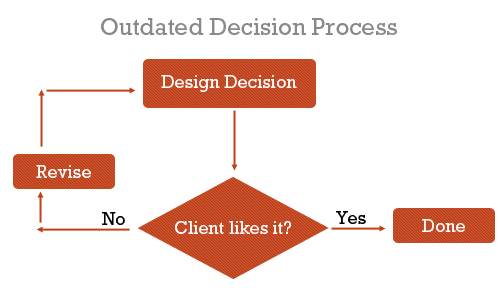
\includegraphics[scale=0.8]{OutDatedDecisionProcess.jpg}
\caption{old decision process, Jacob Gube 2010}
\end{figure}
nowhere in the design process was the users a factor, the design was simply made according to how the designers as well as the client felt it should be. making the same kind of chart for a user-centered approach would look differently:\\
\begin{figure}[H]
\centering
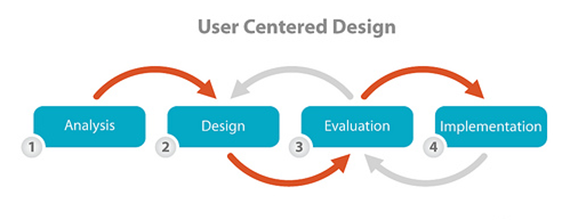
\includegraphics[scale=0.8]{UserCenteredDesign.png}
\caption{a chart of how user-centered design could function, Usabilla 2014}
\end{figure}
as this chart shows, user-centered design can be an iterative process. the grey arrow represents the user feedback, which shows that the users should be involved in the evaluation of a design. This method can be overwhelming if the evaluation is only being done on implemented prototypes\todo{source}.

User Experience and usability is often confused since a large portion of the guidelines for proper usability also applies to giving a good user experience. What sets the user experience apart from usability is the feelings that the user is subjected to while using the site, app or programme.
\todo{source for the example}An example of which could be the iBooks app for iPad, which is basically an application for reading and browsing E-books. The layout is simple,  it provides an overview of the owned books with a visual representation of the covers which is common for such apps and as such, do not set itself apart from the state of the art when it comes to usability, however the user experience is greatly improved simply by changing the background to resemble a bookshelf, it gives a "cozy" feel to the app, you can almost imagine yourself sitting in front of the fireplace sitting with a good book.
\begin{figure}[H]
\centering
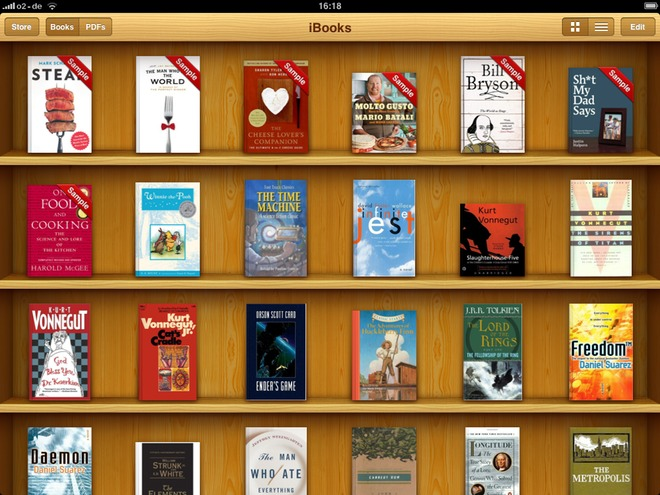
\includegraphics[scale=0.5]{iBooks.png}
\caption{Apple iBooks for comparison}
\end{figure}

\begin{figure}[H]
\centering
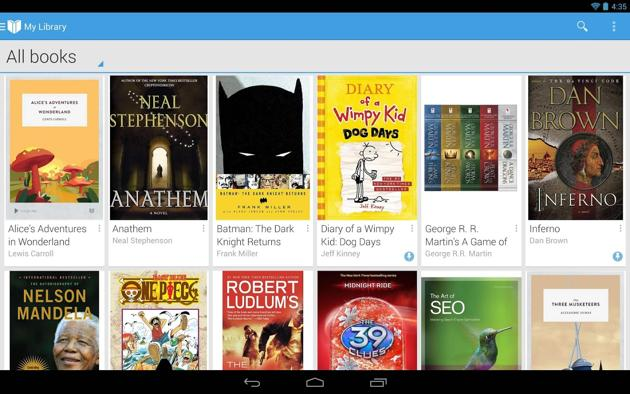
\includegraphics[scale=0.5]{GooglePlayBooks.png}
\caption{Google Play Books for comparison}
\end{figure}
<<<<<<< HEAD
<<<<<<< HEAD
=======


>>>>>>> parent of b7d1b95... Todays work on UX plus extra check description
=======


>>>>>>> parent of b7d1b95... Todays work on UX plus extra check description
\subsection{User experience for mobiles}
when designing a mobile app with UX focus, the unique challenges of the mobile platform has to be considered. A brief look at three of the most outstanding challenges:
\begin{itemize}
\item Screen size\\
as opposed to a traditional computer screen the general mobile platform has a much more limited amount of screen space. This restriction will force the designers to eliminate as many redundancies as possible so as to not clutter the screen with unnecessary information. \cite{Sardo}
\item User input\\
user input is according to Giorgio Sardo one of  the smartphones weakness. it is mentioned that “Entering text on a mobile phone is hard, and people tend to avoid it if they can”\cite{Sardo}
\item Loading times\\
Mobile devices are generally slower than a PC or Mac, both when it comes to processing power and internet speed, assuming they’re using a mobile network \cite{MobileUsability}
\end{itemize}
When attempting to improve usability and user experience, for people using a site or a programme on a phone, the optimal way to do so is to make an actual app where you either port the mobile site or the web application so that it can be downloaded and accessed directly from your phone or tablet instead of via the internet browser. 
Some of the guidelines for optimizing for mobile devices are cutting features, reduce word count and enlarge interface elements to accommodate the “fat finger problem”.\cite{MobileUsability} an example of poor simplification used in the book is IKEA where they simplify the mobile site by only showing a single item when browsing for bedframes.

\begin{figure}[H]
\centering
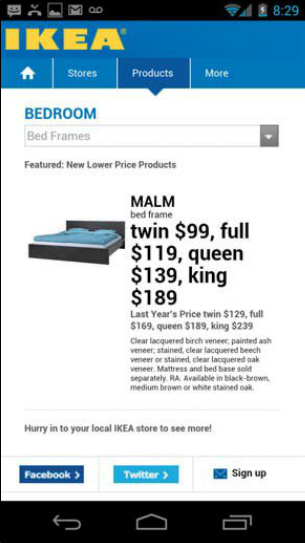
\includegraphics[scale=0.5]{IkeaBadMobile.png}
\caption{the mobile website from IKEA, anno 2013}
\end{figure}

\subsection{Understanding our Users}
Even though we have previously analysed out target group, when we want to focus on the user experience, further target group considerations has to be made, that is why this paper will next talk about the concept of understanding the users. Georgi Sardo provides three points that will help with the design process of the app:
\begin{itemize}
\item What are your users’ digital device skills? Are they used to working with digital devices and software applications?\cite{Sardo}
\item What are your users’ skills in using your application? Does the application revolve around their professional area?\cite{Sardo}
\item Is the application the focal point for your users? Or is their attention limited?\cite{Sardo}
\end{itemize}
these three points can help develop an app that will be focused on the users needs, which is at its core what UX is all about.
